%\documentclass[twoside,twocolumn,spanish]{article}
\documentclass{article}
\usepackage{lipsum}
\usepackage[T1]{fontenc}
\usepackage[utf8]{inputenc}
\usepackage{graphicx}
\usepackage[spanish]{babel}
\usepackage{amssymb,amsmath,geometry,multicol,spalign,hyperref}
\setlength\columnsep{20pt}
\usepackage[usenames,dvipsnames]{xcolor}
\usepackage{tikz,mathtools}
\usepackage{circuitikz}
\usepackage{pgfplots}
\pgfplotsset{width=5cm,compat=1.12}
\usepgfplotslibrary{fillbetween}

\title{Cálculo de la constante elástica de un muelle}
\author{Andoni Latorre Galarraga \\ \href{mailto:alatorre73@alumno.uned.es}{alatorre73@alumno.uned.es}}
\date{}
\begin{document}
\maketitle
\begin{abstract}
  Se estudia la relación entre una masa y el periodo de oscilación de esta al ser suspendida de un muelle. A partir de los datos experimentales se calcula el valor de la constante elástica del muelle. El experimento se desarrolla siguiendo el proceso explicado en \cite{web}.
\end{abstract}

\begin{multicols}{2}

\section*{Fundamento Teórico}

La ley de Hooke predice que si se aplica una fuerza $F$ a un muelle la elongación $x$ es proporcional a dicha fuerza.
$$
F = - k x
$$
Donde la constante de proporcionalidad $k$ es la constante elástica del muelle. Si se suspende una masa $M$ del muelle, aplicando la segunda ley de Newton, se tiene
$$
Ma=-kx \Rightarrow \frac{d^2x}{dt^2} = -\frac{k}{M} x
$$
De la solución de la ecuación diferencial, $C_1\sen(\sqrt{\frac{k}{M}} t) + C_2\cos(\sqrt{\frac{k}{M}} t)$, se deduce el periodo de oscilación, $T$.
$$
T = 2\pi \sqrt{\frac{M}{k}}
$$
\begin{center}
\begin{circuitikz}
  \draw (0,0) to[spring, l=$k$] (0,1.25);
  \draw[fill=gray!40] (-.25,0) rectangle (.25,-.5);
  \node at (0,-0.25) {$M$};
  \draw[-stealth, thick] (0,-.5) -- (0,-1.5);
  \node at (.25,-1) {$F$};
\end{circuitikz}
\end{center}
Para considerar la masa del muelle, $m$, como toda la masa del muelle no está tan desplazada, se le suma a la masa una cantidad $\alpha m$ con $\alpha <1$.
$$
T = 2\pi \sqrt{\frac{M+\alpha m}{k}}
$$
Tomado cuadrados obtenemos una relación lineal entre $T^2$ y $M$ (resaltados es azul).
$$
\textcolor{blue}{T^2} = \frac{4\pi^2}{K} \textcolor{blue}{M} + \frac{4\pi^2\alpha m}{K}
$$
Estudiaremos la pendiente para obtener el valor de $k$.

\section*{Dispositivo experimental}

El dispositivo experimental consiste en un muelle del cual se ha suspendido un soporte en el cual se pueden colocar distintas masas. En la Fig. 1 se puede observa el dispositivo experimental.
\begin{center}
  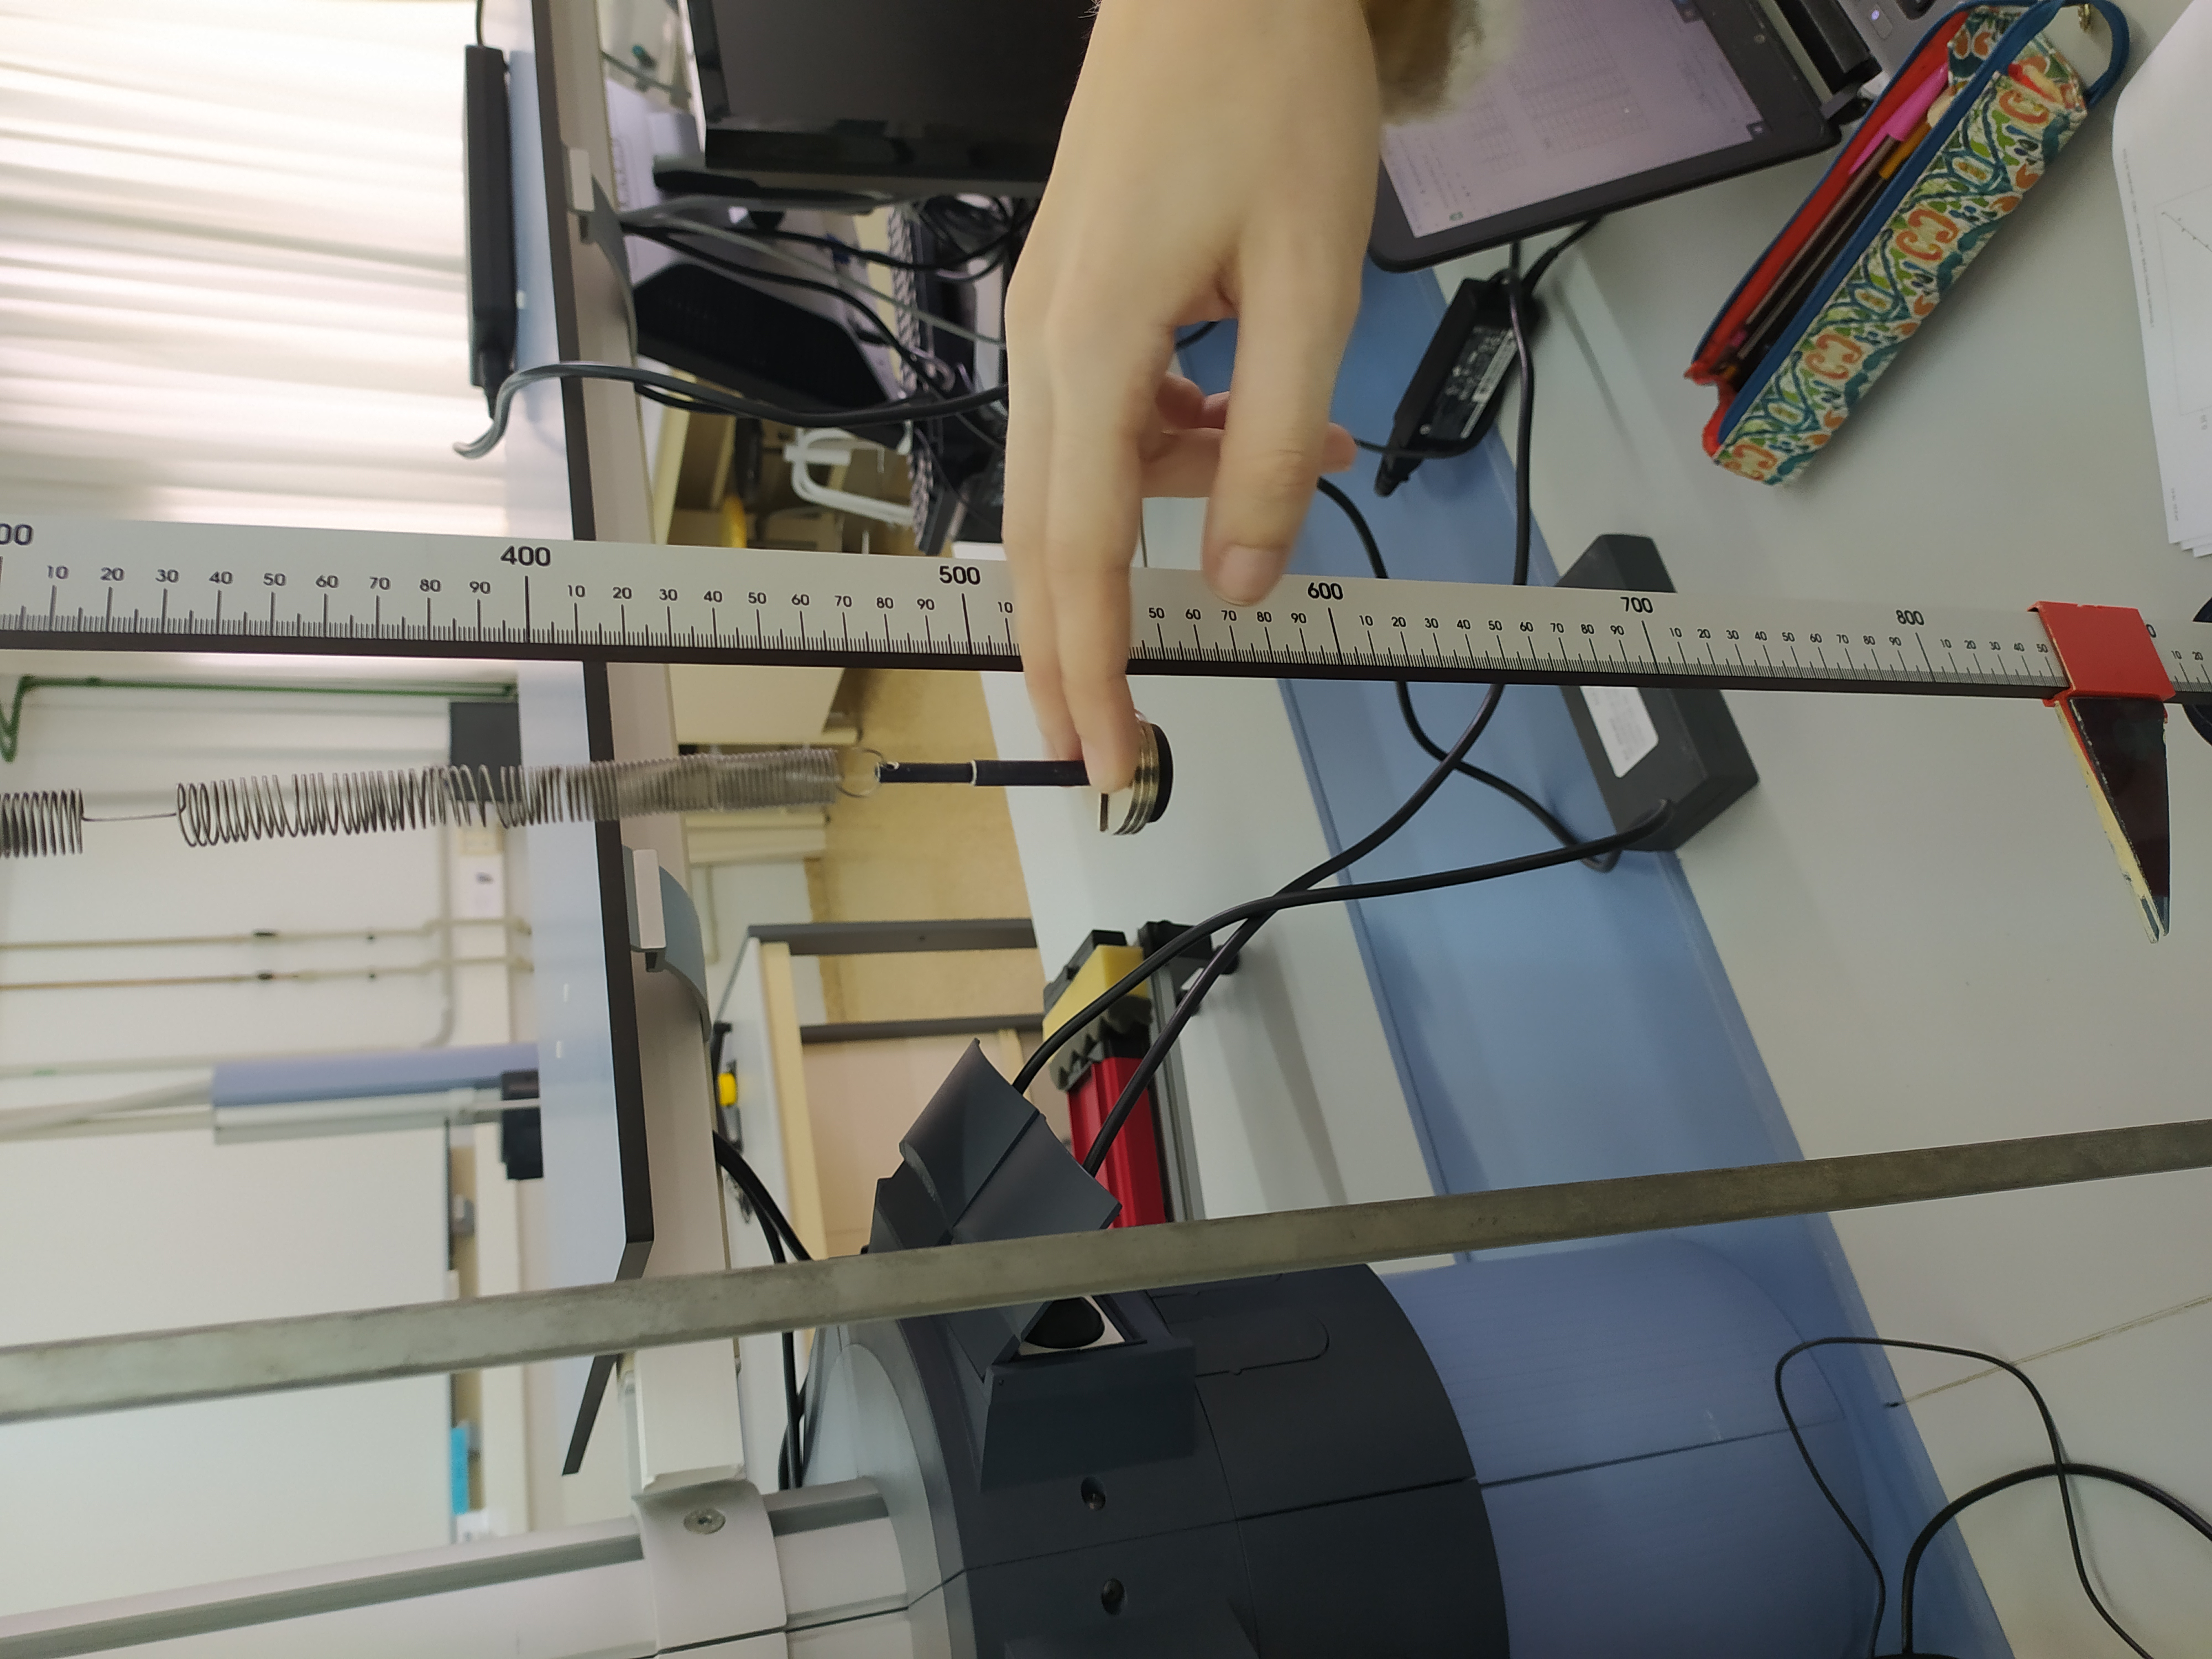
\includegraphics[scale=0.06, angle=-90, trim={500 0 1600 0}, clip]{figures/muelle_montado.jpg}\\
  Figura 1: Dispositivo experimental.
\end{center}
Al lado de muelle y el soporte se encuentra una escala con precisión de 1mm con un plástico (ver Fig. 2) para asistir en la medición.
\begin{center}
  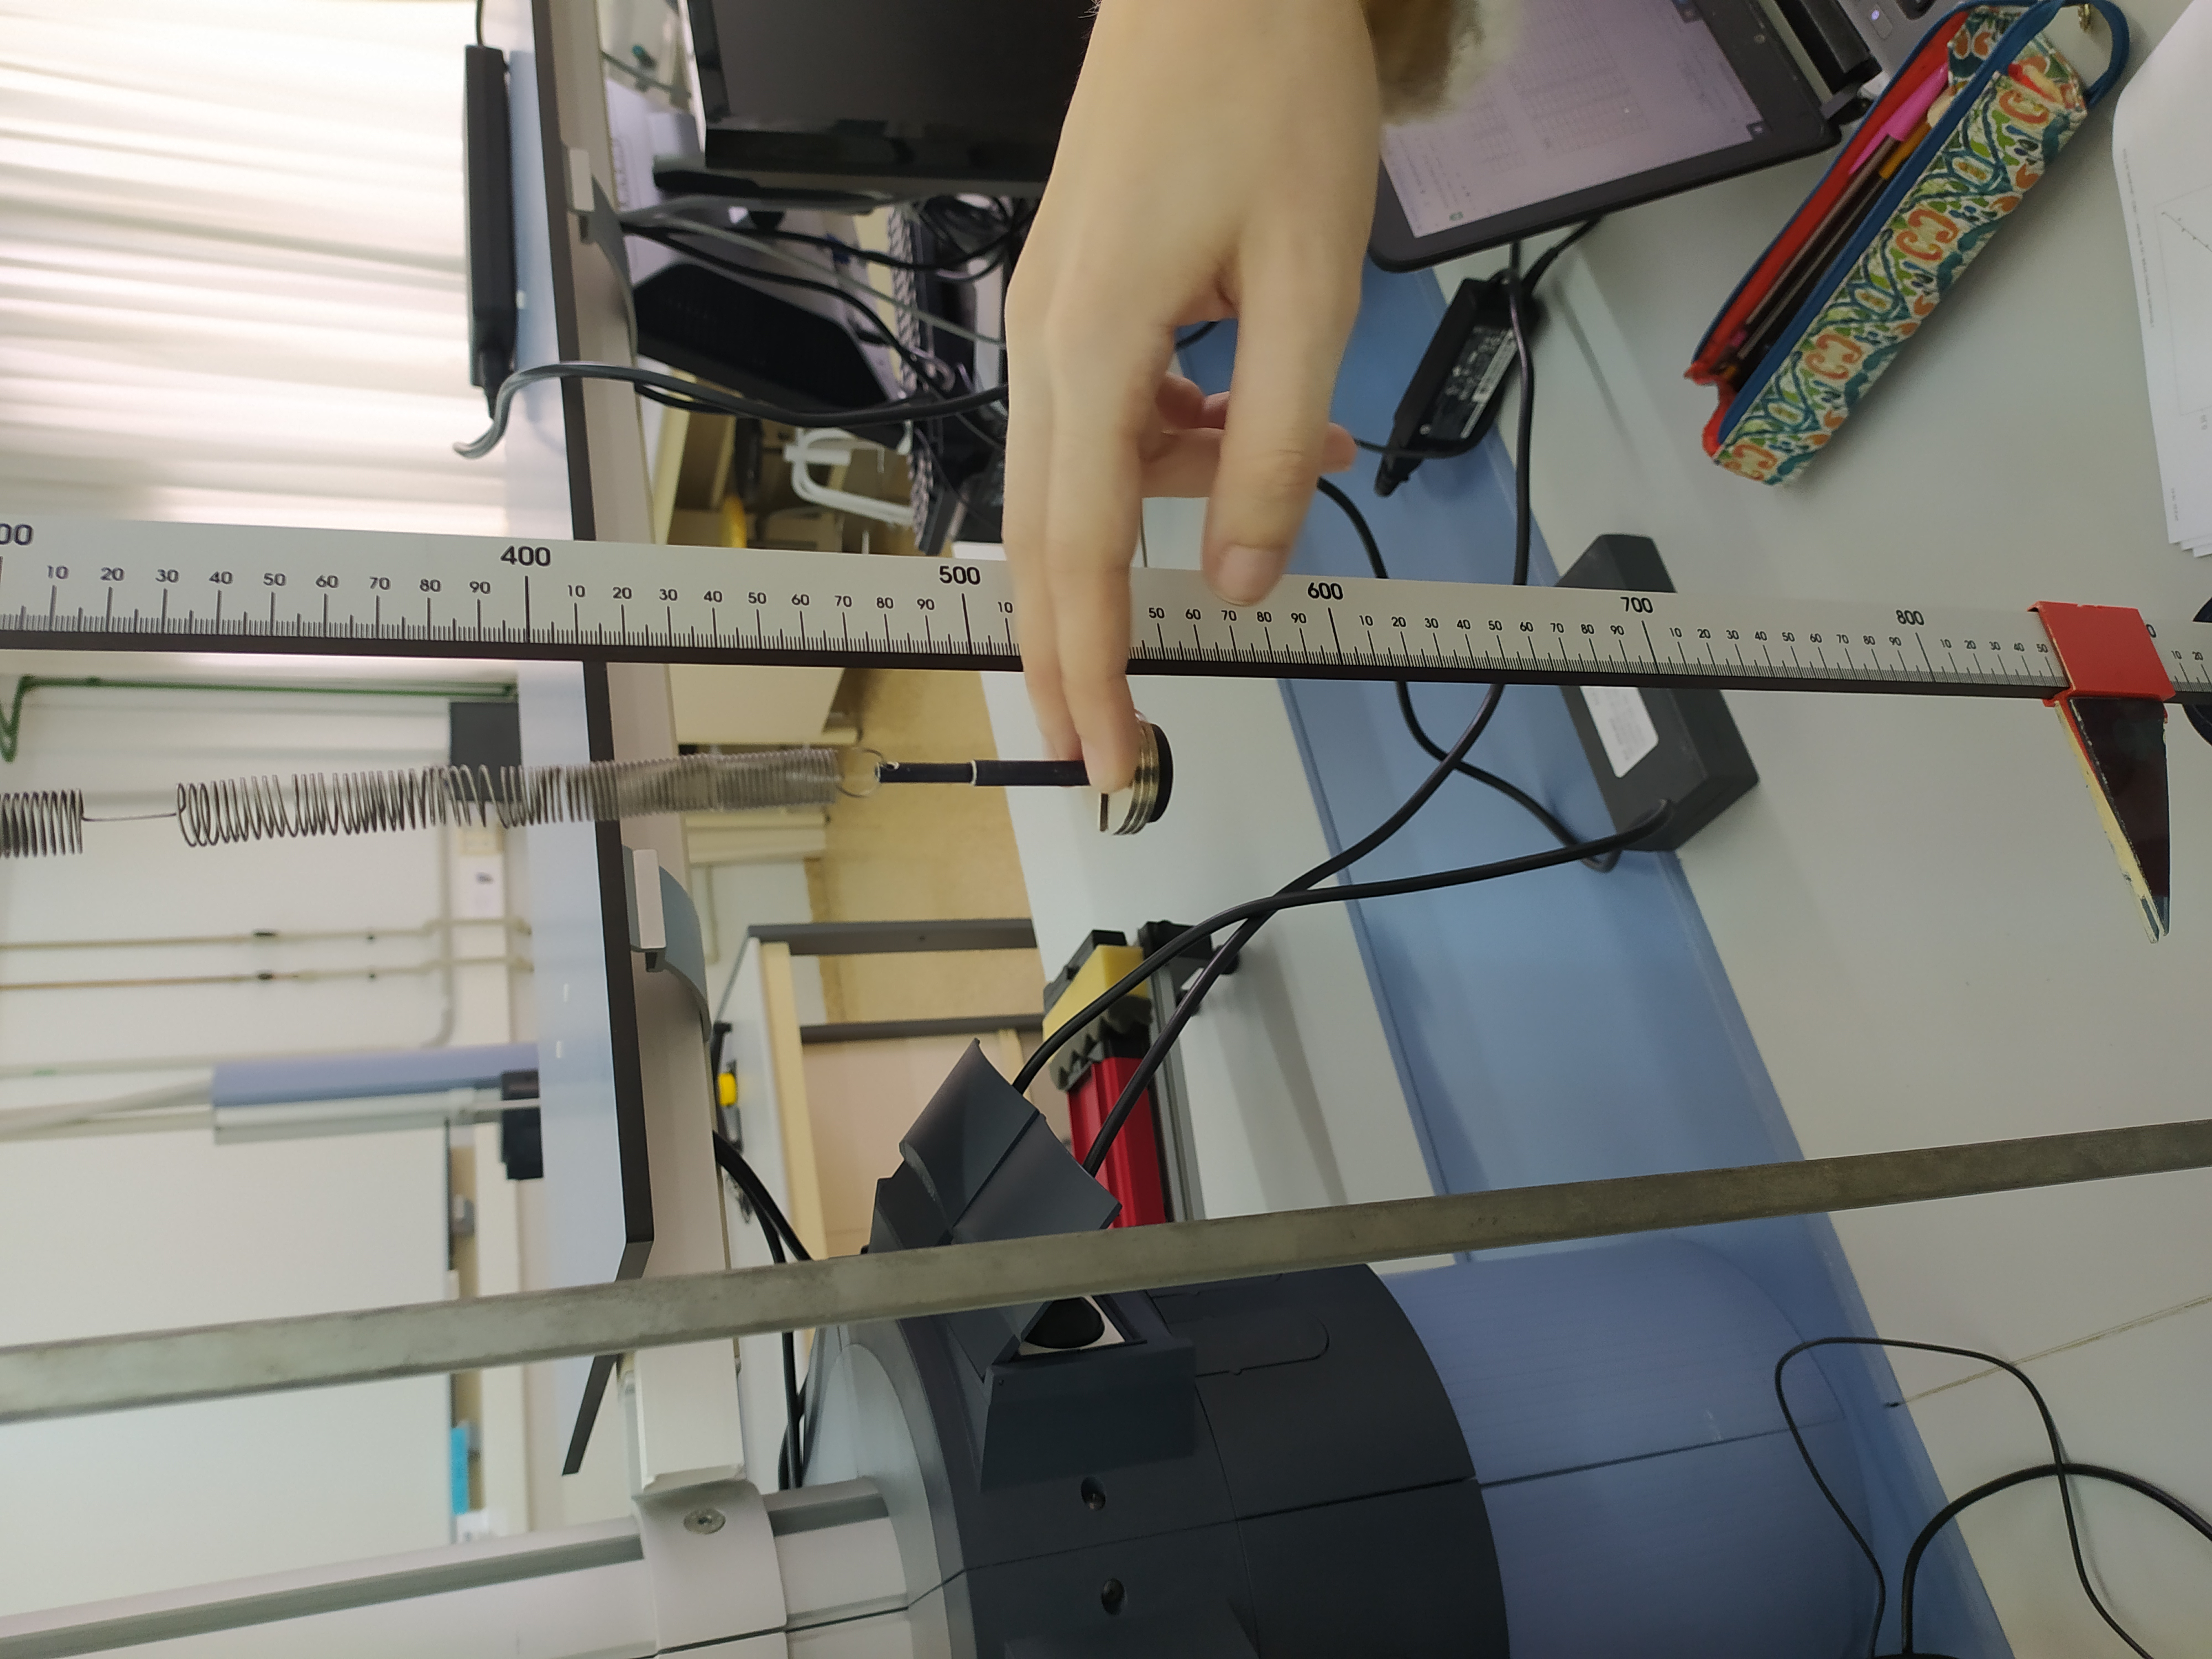
\includegraphics[scale=0.06, angle=-90, trim={3000 0 0 0}, clip]{figures/muelle_montado.jpg}\\
  Figura 2: Plástico unido a la escala vertical para asistir con las mediciones.
\end{center}

\section*{Procedimiento y Resultados}

Para una primera estimación del valor del valor de $k$ utilizaremos la relación lineal entre la fuerza y la elongación.
$$
 F = Mg = -kx
$$
Para el valor de $g$ tomaremos será de $-9,847$ms\textsuperscript{-2}, obtenido de \cite{gravedad} sabiendo que la latitud del laboratorio es de unos $43.3305^\circ$. Para obtener el error de $F$, utilizamos propagación cuadrática.
$$
\epsilon_F = \sqrt{\left| \frac{dF}{dM} \right|^2 \epsilon_M^2 } = g \epsilon_M
$$
Los datos experimentales son los siguientes:
\begin{center}
Tabla 1:
$$
\begin{array}{|l|l|l|l|l|l|} \hline
  x\text{(m)} & \epsilon_x\text{(m)} & M\text{(kg)} & \epsilon_M\text{(Kg)} & F\text{(N)} & \epsilon_F\text{(N)} \\ \hline \hline
  0.007 & 0.001 & 0.01 & 0.002 & -0.10 & 0.02  \\ \hline
  0.013 & 0.001 & 0.02 & 0.002 & -0.20 & 0.02  \\ \hline
  0.019 & 0.001 & 0.03 & 0.002 & -0.30 & 0.02  \\ \hline
  0.026 & 0.001 & 0.04 & 0.002 & -0.39 & 0.02  \\ \hline
  0.031 & 0.001 & 0.05 & 0.002 & -0.49 & 0.02  \\ \hline
  0.037 & 0.001 & 0.06 & 0.002 & -0.59 & 0.02  \\ \hline
  0.044 & 0.001 & 0.07 & 0.002 & -0.69 & 0.02  \\ \hline
  0.050 & 0.001 & 0.08 & 0.002 & -0.79 & 0.02  \\ \hline
  0.056 & 0.001 & 0.09 & 0.002 & -0.89 & 0.02  \\ \hline
  0.064 & 0.001 & 0.10 & 0.002 & -0.98 & 0.02  \\ \hline
  0.071 & 0.001 & 0.11 & 0.002 & -1.08 & 0.02  \\ \hline
  0.077 & 0.001 & 0.12 & 0.002 & -1.18 & 0.02  \\ \hline
  0.083 & 0.001 & 0.13 & 0.002 & -1.28 & 0.02  \\ \hline
  0.090 & 0.001 & 0.14 & 0.002 & -1.38 & 0.02  \\ \hline
\end{array}
$$
$$
  \begin{array}{|l|l|l|l|l|l|} \hline
  x\text{(m)} & \epsilon_x\text{(m)} & M\text{(kg)} & \epsilon_M\text{(Kg)} & F\text{(N)} & \epsilon_F\text{(N)} \\ \hline \hline
  0.093 & 0.001 & 0.15 & 0.002 & -1.48 & 0.02  \\ \hline
  0.099 & 0.001 & 0.16 & 0.002 & -1.58 & 0.02  \\ \hline
  0.106 & 0.001 & 0.17 & 0.002 & -1.67 & 0.02  \\ \hline
  0.111 & 0.001 & 0.18 & 0.002 & -1.77 & 0.02  \\ \hline
  0.118 & 0.001 & 0.19 & 0.002 & -1.87 & 0.02  \\ \hline
  \end{array}
$$
\end{center}
En la Fig. 3 se muestra la fuerza, $F$, frente a la elongación, $x$ junto con la recta de regresión.
\begin{center}
  \includegraphics[width = 0.45\textwidth]{figures/regresión1.png}\\
  Figura 3: $F$ frente a $x$ junto con la recta de regresión.
\end{center}
De la pendiente de la recta de regresión deducimos que
$$
-k = (-15.83 \pm 0.13 ) \text{ kg s}^{-2}
$$
$$
\Rightarrow k = (15.83 \pm 0.13 ) \text{ kg s}^{-2}
$$
Por otra parte también estimaremos el valor de $k$ a traves de la relación lineal.
$$
T^2 = \frac{4\pi^2}{K} M + \frac{4\pi^2\alpha m}{K}
$$
Se han tomado 4 tiempos para 10 oscilaciones con 12 masas diferentes. Los datos experimentales son:
\begin{center}
Tabla 2:
$$
\begin{array}{|l|l|l|l|l|} \hline
  m\text{(kg)} & T_1\text{(s)} & T_2\text{(s)} & T_3\text{(s)} & T_4\text{(s)} \\ \hline \hline
  0,03 & 3,69 & 3,69 & 3,90 & 3,59  \\ \hline
  0,04 & 3,94 & 3,90 & 3,91 & 3,93  \\ \hline
  0,05 & 4,28 & 4,25 & 4,33 & 4,25  \\ \hline
  0,06 & 4,47 & 4,41 & 4,50 & 4,56  \\ \hline
  0,07 & 4,75 & 4,81 & 4,65 & 4,88  \\ \hline
  0,08 & 4,94 & 4,97 & 4,88 & 4,94  \\ \hline
\end{array}
$$
$$
\begin{array}{|l|l|l|l|l|} \hline
  m\text{(kg)} & T_1\text{(s)} & T_2\text{(s)} & T_3\text{(s)} & T_4\text{(s)} \\ \hline \hline
  0,09 & 5,22 & 5,25 & 5,25 & 5,00  \\ \hline
  0,10 & 5,50 & 5,59 & 5,68 & 5,50  \\ \hline
  0,12 & 5,88 & 5,91 & 5,93 & 5,81  \\ \hline
  0,15 & 6,50 & 6,65 & 6,59 & 6,50  \\ \hline
  0,17 & 6,97 & 6,94 & 6,94 & 6,97  \\ \hline
  0,20 & 7,32 & 7,38 & 7,44 & 7,44  \\ \hline
  \end{array}
$$
\end{center}
Primero calcularemos la media de los 4 tiempos:
$$
\overline{T} = \frac{1}{4}\sum_{i=1}^4 T_i
$$
Y para su error calcularemos la dispersión de los 4 tiempos como se indica en la ecuación (2.5) de \cite{manual}.
$$
D = \frac{\max_i T_i - \min_i T_i}{2}
$$
Y luego el error de acuerdo con la fórmula (2.8) de \cite{manual}.
$$
\epsilon_{\overline{T}} = \frac{D}{\sqrt{4}}
$$
$$
\Rightarrow
\epsilon_{\overline{T}} = \frac{\max_i T_i - \min_i T_i}{4}
$$
Ahora como $\overline{T} = 10 T$ Podemos calcular $T$ y su error.
$$
T = \frac{\overline{T}}{10}
$$
$$
\epsilon_T = \sqrt{\left| \frac{dT}{d\overline{T}} \right|^2 \epsilon_{\overline{T}}^2 } = \frac{\epsilon_{\overline{T}}}{10}
$$
$$
\Rightarrow
T = \frac{1}{40}\sum_{i=1}^4 T_i \quad \epsilon_{T} = \frac{\max_i T_i - \min_i T_i}{40}
$$
De nuevo, aplicando la propagación cuadrática de errores para $T^2$,
$$
\epsilon_{T^2} = 2T\epsilon_T
$$
\begin{center}
Tabla 3:  
$$
\begin{array}{|l|l|l|l|l|} \hline
  M\text{(kg)} & T\text{(s)} & \epsilon_T\text{(s)} & T^2\text{(s\textsuperscript{2})} & \epsilon_{T^2}\text{(s\textsuperscript{2})}\\ \hline \hline
  0.03 & 0.372 & 0.008 & 0.138 & 0.006  \\ \hline
  0.04 & 0.3920 & 0.0010 & 0.1537 & 0.0008  \\ \hline
  0.05 & 0.428 & 0.002 & 0.183 & 0.0017  \\ \hline
  0.06 & 0.448 & 0.004 & 0.201 & 0.003  \\ \hline
  0.07 & 0.477 & 0.006 & 0.228 & 0.005  \\ \hline
  0.08 & 0.493 & 0.002 & 0.243 & 0.002  \\ \hline
  0.09 & 0.517 & 0.006 & 0.267 & 0.006  \\ \hline
  0.10 & 0.557 & 0.004 & 0.31 & 0.005  \\ \hline
  0.12 & 0.588 & 0.003 & 0.346 & 0.004  \\ \hline
  0.15 & 0.656 & 0.004 & 0.43 & 0.005  \\ \hline
  0.17 & 0.6955 & 0.0007 & 0.4837 & 0.001  \\ \hline
  0.20 & 0.740 & 0.003 & 0.547 & 0.004  \\ \hline
  \end{array}
$$
\end{center}
En la Fig. 4 se pude ver $T^2$ frente a $M$ junto con la recta de regresión.
\begin{center}
  \includegraphics[width = 0.45\textwidth]{figures/regresión2.png}\\
  Figura 4: $T^2$ frente a $M$ junto con la recta de regresión $y = ax+b$.
  $$
  a = (2.47 \pm 0.04) \text{ s\textsuperscript{2} kg\textsuperscript{-1}}
  $$
  $$
  b = (0.055 \pm 0.004) \text{ s\textsuperscript{2}}
  $$
\end{center}
Sabiendo la pendiente de la recta calculamos la constante elástica y su error.
$$
k = \frac{4\pi^2}{a}
$$
$$
\epsilon_k = \sqrt{\left| \frac{dk}{da} \right|^2 \epsilon_a^2} = \frac{4\pi^2}{a^2} \epsilon_a
$$
$$
k= (16.0 \pm 0.3) \text{ kg s}^{-2}
$$
A partir de la ordenada en el origen, se puede calcular $\alpha m$ y su error.
$$
b = \frac{4\pi^2}{K} \alpha m = a \alpha m
$$
$$
\Rightarrow \alpha m = \frac{b}{a}
$$
$$
\epsilon_{\alpha m} = \sqrt{\left| \frac{\partial \alpha m}{\partial a} \right|^2 \epsilon_a^2 + \left| \frac{\partial \alpha m}{\partial b} \right|^2 \epsilon_b^2}
$$
$$
= \sqrt{\left(\frac{-b}{a^2}\right)^2 \epsilon_a^2 + \left( \frac{1}{a}\right)^2 \epsilon_b^2} = 
\frac{1}{a}\sqrt{b^2 \epsilon_b^2 + \epsilon_a^2}
$$
$$
\alpha m = (0.022 \pm 0.016) \text{ kg}
$$
$$
\alpha m = (22 \pm 16) \text{ g}
$$
Este resulado es muy impreciso, ya que tiene un error relativo de más del 70\%. A partir de consideraciones energeticas, como se indica en \cite{web} se puede calcular el valor de $\alpha$, que debe de ser $\frac{1}{3}$. Sabiendo esto podemos calcular $m$ y su error.
$$
m = 3 \alpha m \quad \epsilon_m = 3 \epsilon_{\alpha m}
$$
$$
m = (70 \pm 50) \text{ g}
$$
\section*{Conclusiones}

El primer valor de $k$, $(15.83 \pm 0.13 ) \text{ kg s}^{-2}$ tiene un error relativo de menos del 1\% y el segundo valor $(16.0 \pm 0.3 ) \text{ kg s}^{-2}$ tiene un error menor al 2\%. Ambos valores son muy precisos y coinciden, ya que existen valores dentro de ambas barras de error. Podemos unficar estos valores utilizando las ecuanciones de \cite{manual} p. 51-52., tomamos una media ponderada donde los pesos están relacionados con los errores de las medidas, dando más peso a las más precisas.
$$
k = \frac{\frac{1}{0,13^2}15,83 + \frac{1}{0,3^2}16,0}{\frac{1}{0,13^2}+\frac{1}{0,3^2}}
$$
$$
\epsilon_k = \frac{1}{\sqrt{\frac{1}{0,13^2}+\frac{1}{0,3^2}}}
$$
$$
k = (15.86\pm 0.12) \text{ kg s}^{-2}
$$
El valor de $m$ es muy impreciso, tiene un error de más del 70\%, además al pesar el muelle directamente se tiene una masa de $(22,9 \pm 0,1) \text{ g}$. Este valor está dentro de la barra de error de la masa obtenida $(70 \pm 50) \text{ g}$, pero está en un extremo del intervalo. El valor de $\alpha$ también puede diferir significativamente del teoríco ya que el muelle presentaba grandes deformaciones, aún así, el valor de $\alpha m$ ya tenia un error relativo inaceptable (72\%). El único valor experimental que se puede considerar es el de $k$, tiene un error relativo pequeño y se han conseguido dos valores compatibles por métodos diferentes. El valor unificado $k = (15.86\pm 0.12) \text{ kg s}^{-2}$ es la mejor predicción experimental del valor real de la constante elástica, tiene un error del 0,76\%.
\begin{thebibliography}{1}

  \bibitem{manual}Manual de la asignatura. Versión 3.7

  \bibitem{web}\url{https://uned-labo.netlify.app/practicas/te/2_practica_ley_hooke/prak2.html} 14/6/2022

  \bibitem{gravedad}\url{https://www.sensorsone.com/local-gravity-calculator/} 14/6/2022

\end{thebibliography}
\end{multicols}
\end{document}